\documentclass[twoside]{book}

% Packages required by doxygen
\usepackage{fixltx2e}
\usepackage{calc}
\usepackage{doxygen}
\usepackage[export]{adjustbox} % also loads graphicx
\usepackage{graphicx}
\usepackage[utf8]{inputenc}
\usepackage{makeidx}
\usepackage{multicol}
\usepackage{multirow}
\PassOptionsToPackage{warn}{textcomp}
\usepackage{textcomp}
\usepackage[nointegrals]{wasysym}
\usepackage[table]{xcolor}

% Font selection
\usepackage[T1]{fontenc}
\usepackage[scaled=.90]{helvet}
\usepackage{courier}
\usepackage{amssymb}
\usepackage{sectsty}
\renewcommand{\familydefault}{\sfdefault}
\allsectionsfont{%
  \fontseries{bc}\selectfont%
  \color{darkgray}%
}
\renewcommand{\DoxyLabelFont}{%
  \fontseries{bc}\selectfont%
  \color{darkgray}%
}
\newcommand{\+}{\discretionary{\mbox{\scriptsize$\hookleftarrow$}}{}{}}

% Page & text layout
\usepackage{geometry}
\geometry{%
  a4paper,%
  top=2.5cm,%
  bottom=2.5cm,%
  left=2.5cm,%
  right=2.5cm%
}
\tolerance=750
\hfuzz=15pt
\hbadness=750
\setlength{\emergencystretch}{15pt}
\setlength{\parindent}{0cm}
\setlength{\parskip}{3ex plus 2ex minus 2ex}
\makeatletter
\renewcommand{\paragraph}{%
  \@startsection{paragraph}{4}{0ex}{-1.0ex}{1.0ex}{%
    \normalfont\normalsize\bfseries\SS@parafont%
  }%
}
\renewcommand{\subparagraph}{%
  \@startsection{subparagraph}{5}{0ex}{-1.0ex}{1.0ex}{%
    \normalfont\normalsize\bfseries\SS@subparafont%
  }%
}
\makeatother

% Headers & footers
\usepackage{fancyhdr}
\pagestyle{fancyplain}
\fancyhead[LE]{\fancyplain{}{\bfseries\thepage}}
\fancyhead[CE]{\fancyplain{}{}}
\fancyhead[RE]{\fancyplain{}{\bfseries\leftmark}}
\fancyhead[LO]{\fancyplain{}{\bfseries\rightmark}}
\fancyhead[CO]{\fancyplain{}{}}
\fancyhead[RO]{\fancyplain{}{\bfseries\thepage}}
\fancyfoot[LE]{\fancyplain{}{}}
\fancyfoot[CE]{\fancyplain{}{}}
\fancyfoot[RE]{\fancyplain{}{\bfseries\scriptsize Generated by Doxygen }}
\fancyfoot[LO]{\fancyplain{}{\bfseries\scriptsize Generated by Doxygen }}
\fancyfoot[CO]{\fancyplain{}{}}
\fancyfoot[RO]{\fancyplain{}{}}
\renewcommand{\footrulewidth}{0.4pt}
\renewcommand{\chaptermark}[1]{%
  \markboth{#1}{}%
}
\renewcommand{\sectionmark}[1]{%
  \markright{\thesection\ #1}%
}

% Indices & bibliography
\usepackage{natbib}
\usepackage[titles]{tocloft}
\setcounter{tocdepth}{3}
\setcounter{secnumdepth}{5}
\makeindex

% Hyperlinks (required, but should be loaded last)
\usepackage{ifpdf}
\ifpdf
  \usepackage[pdftex,pagebackref=true]{hyperref}
\else
  \usepackage[ps2pdf,pagebackref=true]{hyperref}
\fi
\hypersetup{%
  colorlinks=true,%
  linkcolor=blue,%
  citecolor=blue,%
  unicode%
}

% Custom commands
\newcommand{\clearemptydoublepage}{%
  \newpage{\pagestyle{empty}\cleardoublepage}%
}

\usepackage{caption}
\captionsetup{labelsep=space,justification=centering,font={bf},singlelinecheck=off,skip=4pt,position=top}

%===== C O N T E N T S =====

\begin{document}

% Titlepage & ToC
\hypersetup{pageanchor=false,
             bookmarksnumbered=true,
             pdfencoding=unicode
            }
\pagenumbering{alph}
\begin{titlepage}
\vspace*{7cm}
\begin{center}%
{\Large Juego Reversi }\\
\vspace*{1cm}
{\large Generated by Doxygen 1.8.14}\\
\end{center}
\end{titlepage}
\clearemptydoublepage
\pagenumbering{roman}
\tableofcontents
\clearemptydoublepage
\pagenumbering{arabic}
\hypersetup{pageanchor=true}

%--- Begin generated contents ---
\chapter{Hierarchical Index}
\section{Class Hierarchy}
This inheritance list is sorted roughly, but not completely, alphabetically\+:\begin{DoxyCompactList}
\item \contentsline{section}{Computadora}{\pageref{class_computadora}}{}
\item \contentsline{section}{Controlador\+Puntajes}{\pageref{class_controlador_puntajes}}{}
\item Serializable\begin{DoxyCompactList}
\item \contentsline{section}{Puntaje}{\pageref{class_puntaje}}{}
\end{DoxyCompactList}
\item \contentsline{section}{Tablero}{\pageref{class_tablero}}{}
\item J\+Frame\begin{DoxyCompactList}
\item \contentsline{section}{Interfaz\+Grafica}{\pageref{class_interfaz_grafica}}{}
\item \contentsline{section}{Menu\+Principal}{\pageref{class_menu_principal}}{}
\item \contentsline{section}{Menu\+Puntajes}{\pageref{class_menu_puntajes}}{}
\item \contentsline{section}{Menu\+Tableros}{\pageref{class_menu_tableros}}{}
\item \contentsline{section}{Puntajes\+Computadora\+O\+Jugador}{\pageref{class_puntajes_computadora_o_jugador}}{}
\end{DoxyCompactList}
\end{DoxyCompactList}

\chapter{Class Index}
\section{Class List}
Here are the classes, structs, unions and interfaces with brief descriptions\+:\begin{DoxyCompactList}
\item\contentsline{section}{\mbox{\hyperlink{class_computadora}{Computadora}} \\*Colección de estrategias para la computadora }{\pageref{class_computadora}}{}
\item\contentsline{section}{\mbox{\hyperlink{class_controlador_puntajes}{Controlador\+Puntajes}} \\*Automatiza el manejo de los archivos de puntajes }{\pageref{class_controlador_puntajes}}{}
\item\contentsline{section}{\mbox{\hyperlink{class_interfaz_grafica}{Interfaz\+Grafica}} \\*Esta clase muestra el tablero y permite jugar en el Cuenta con los modos de juego con computadora y 2 jugadores Esta es un frame y recibe interaccion con el usuario mediante el mouse. Este ultimo es el que tiene la informacion de cuando se termina el juego y realiza las operaciones de poner fichas }{\pageref{class_interfaz_grafica}}{}
\item\contentsline{section}{\mbox{\hyperlink{class_menu_principal}{Menu\+Principal}} \\*La clase del menu principal es la que contiene el main Esta cuenta con las opciones para jugar dso jugadores o solo contra la computadora. Tambien tiene la opcion de entrar a los puntajes y salir del juego }{\pageref{class_menu_principal}}{}
\item\contentsline{section}{\mbox{\hyperlink{class_menu_puntajes}{Menu\+Puntajes}} \\*Este es el menu que contiene los puntajes cuenta con los botones muestra en la pantalla los puntajes de los 3 distintos tableros }{\pageref{class_menu_puntajes}}{}
\item\contentsline{section}{\mbox{\hyperlink{class_menu_tableros}{Menu\+Tableros}} \\*Esta clase muestra las opciones de los 3 tableros para elegir en cual jugar }{\pageref{class_menu_tableros}}{}
\item\contentsline{section}{\mbox{\hyperlink{class_puntaje}{Puntaje}} \\*Información de una fila en cada tabla de puntajes }{\pageref{class_puntaje}}{}
\item\contentsline{section}{\mbox{\hyperlink{class_puntajes_computadora_o_jugador}{Puntajes\+Computadora\+O\+Jugador}} }{\pageref{class_puntajes_computadora_o_jugador}}{}
\item\contentsline{section}{\mbox{\hyperlink{class_tablero}{Tablero}} \\*El tablero donde se almacena la información del juego }{\pageref{class_tablero}}{}
\end{DoxyCompactList}

\chapter{Class Documentation}
\hypertarget{class_computadora}{}\section{Computadora Class Reference}
\label{class_computadora}\index{Computadora@{Computadora}}


Colección de estrategias para la computadora.  


\subsection*{Public Member Functions}
\begin{DoxyCompactItemize}
\item 
\mbox{\hyperlink{class_computadora_ad4355373f2816ef2eb5d725283e632b4}{Computadora}} (\mbox{\hyperlink{class_tablero}{Tablero}} tablero, int estrategia, int color)
\begin{DoxyCompactList}\small\item\em Construye una instancia de \mbox{\hyperlink{class_computadora}{Computadora}} que trabaja con el tablero, estrategia y color indicado. \end{DoxyCompactList}\item 
void \mbox{\hyperlink{class_computadora_a935c14f6094fc48b44a3dc789892a522}{jugada}} ()
\begin{DoxyCompactList}\small\item\em Realiza una juada. \end{DoxyCompactList}\end{DoxyCompactItemize}


\subsection{Detailed Description}
Colección de estrategias para la computadora. 

Cada instancia se debe construir especificando sobre cuál tablero debe jugar, qué estrategia debe usar y cuál color usa.

Para que la computadora realice una jugada, se debe invocar al método \mbox{\hyperlink{class_computadora_a935c14f6094fc48b44a3dc789892a522}{jugada()}}.

Actualmente existen dos estrategias\+:
\begin{DoxyItemize}
\item La estrategia número 0 pone la ficha en el primer lugar que encuentra, buscando de derecha a izquierda y de arriba a abajo.
\item La estrategia no. 1 busca la posición donde pueda comer la mayor cantidad de fichas posible. 
\end{DoxyItemize}

\subsection{Constructor \& Destructor Documentation}
\mbox{\Hypertarget{class_computadora_ad4355373f2816ef2eb5d725283e632b4}\label{class_computadora_ad4355373f2816ef2eb5d725283e632b4}} 
\index{Computadora@{Computadora}!Computadora@{Computadora}}
\index{Computadora@{Computadora}!Computadora@{Computadora}}
\subsubsection{\texorpdfstring{Computadora()}{Computadora()}}
{\footnotesize\ttfamily Computadora.\+Computadora (\begin{DoxyParamCaption}\item[{\mbox{\hyperlink{class_tablero}{Tablero}}}]{tablero,  }\item[{int}]{estrategia,  }\item[{int}]{color }\end{DoxyParamCaption})}



Construye una instancia de \mbox{\hyperlink{class_computadora}{Computadora}} que trabaja con el tablero, estrategia y color indicado. 


\begin{DoxyParams}{Parameters}
{\em tablero} & El tablero sobre el cual debe realizar las jugadas. \\
\hline
{\em estrategia} & El número de la estrategia que debe seguir. \\
\hline
{\em color} & El color con el cual juega. \\
\hline
\end{DoxyParams}


\subsection{Member Function Documentation}
\mbox{\Hypertarget{class_computadora_a935c14f6094fc48b44a3dc789892a522}\label{class_computadora_a935c14f6094fc48b44a3dc789892a522}} 
\index{Computadora@{Computadora}!jugada@{jugada}}
\index{jugada@{jugada}!Computadora@{Computadora}}
\subsubsection{\texorpdfstring{jugada()}{jugada()}}
{\footnotesize\ttfamily void Computadora.\+jugada (\begin{DoxyParamCaption}{ }\end{DoxyParamCaption})}



Realiza una juada. 

Este método debe invocarse cada vez que se desee que la computadora realice una jugada. 

The documentation for this class was generated from the following file\+:\begin{DoxyCompactItemize}
\item 
Computadora.\+java\end{DoxyCompactItemize}

\hypertarget{class_controlador_puntajes}{}\section{Controlador\+Puntajes Class Reference}
\label{class_controlador_puntajes}\index{Controlador\+Puntajes@{Controlador\+Puntajes}}


Automatiza el manejo de los archivos de puntajes.  


\subsection*{Public Member Functions}
\begin{DoxyCompactItemize}
\item 
\mbox{\hyperlink{class_controlador_puntajes_ab192cfbffc96954094f47b5b66e8cda5}{Controlador\+Puntajes}} (String nombre\+Archivo)
\begin{DoxyCompactList}\small\item\em Crea un objeto que automatiza el manejo de puntajes en el archivo indicado. \end{DoxyCompactList}\item 
\mbox{\Hypertarget{class_controlador_puntajes_ad44446c5c7a56f497edf2982d0fcc952}\label{class_controlador_puntajes_ad44446c5c7a56f497edf2982d0fcc952}} 
int {\bfseries get\+Minimo} ()
\item 
void \mbox{\hyperlink{class_controlador_puntajes_a101a964a47c4ed0036f70c3a5c2d58ca}{agregar\+Puntaje}} (\mbox{\hyperlink{class_puntaje}{Puntaje}} p)
\begin{DoxyCompactList}\small\item\em Agrega el puntaje especificado a la lista. \end{DoxyCompactList}\item 
\mbox{\Hypertarget{class_controlador_puntajes_a973c3ca7103da4783b64b46cc716532e}\label{class_controlador_puntajes_a973c3ca7103da4783b64b46cc716532e}} 
\mbox{\hyperlink{class_puntaje}{Puntaje}} {\bfseries get\+Puntaje} (int n)
\item 
\mbox{\Hypertarget{class_controlador_puntajes_a51d112050ac7772fe74bc1290a14f2f3}\label{class_controlador_puntajes_a51d112050ac7772fe74bc1290a14f2f3}} 
String {\bfseries to\+String} ()
\end{DoxyCompactItemize}


\subsection{Detailed Description}
Automatiza el manejo de los archivos de puntajes. 

Esta clase automatiza el manejo de los archivos de puntajes.

Primero se debe inicializar la instancia especificando el nombre del archivo donde se desea trabajar. Esto automáticamente carga los puntajes desde el archivo, y si el archivo no existe, lo crea con una lista vacía.

Una vez cargados los puntajes, se pueden leer mediante el método get\+Puntaje(), y se puede agregar un puntaje mediante \mbox{\hyperlink{class_controlador_puntajes_a101a964a47c4ed0036f70c3a5c2d58ca}{agregar\+Puntaje()}} (que lo coloca ordenado según puntaje y descarta los puntajes que exceden los 10 espacios).

Los puntajes se guardan de vuelta al archivo especificado con cada llamada al método \mbox{\hyperlink{class_controlador_puntajes_a101a964a47c4ed0036f70c3a5c2d58ca}{agregar\+Puntaje()}}. 

\subsection{Constructor \& Destructor Documentation}
\mbox{\Hypertarget{class_controlador_puntajes_ab192cfbffc96954094f47b5b66e8cda5}\label{class_controlador_puntajes_ab192cfbffc96954094f47b5b66e8cda5}} 
\index{Controlador\+Puntajes@{Controlador\+Puntajes}!Controlador\+Puntajes@{Controlador\+Puntajes}}
\index{Controlador\+Puntajes@{Controlador\+Puntajes}!Controlador\+Puntajes@{Controlador\+Puntajes}}
\subsubsection{\texorpdfstring{Controlador\+Puntajes()}{ControladorPuntajes()}}
{\footnotesize\ttfamily Controlador\+Puntajes.\+Controlador\+Puntajes (\begin{DoxyParamCaption}\item[{String}]{nombre\+Archivo }\end{DoxyParamCaption})}



Crea un objeto que automatiza el manejo de puntajes en el archivo indicado. 


\begin{DoxyParams}{Parameters}
{\em nombre\+Archivo} & El nombre del archivo donde se desea trabajar. \\
\hline
\end{DoxyParams}


\subsection{Member Function Documentation}
\mbox{\Hypertarget{class_controlador_puntajes_a101a964a47c4ed0036f70c3a5c2d58ca}\label{class_controlador_puntajes_a101a964a47c4ed0036f70c3a5c2d58ca}} 
\index{Controlador\+Puntajes@{Controlador\+Puntajes}!agregar\+Puntaje@{agregar\+Puntaje}}
\index{agregar\+Puntaje@{agregar\+Puntaje}!Controlador\+Puntajes@{Controlador\+Puntajes}}
\subsubsection{\texorpdfstring{agregar\+Puntaje()}{agregarPuntaje()}}
{\footnotesize\ttfamily void Controlador\+Puntajes.\+agregar\+Puntaje (\begin{DoxyParamCaption}\item[{\mbox{\hyperlink{class_puntaje}{Puntaje}}}]{p }\end{DoxyParamCaption})}



Agrega el puntaje especificado a la lista. 

Agrega el puntaje especificado a la lista, insertándolo en la posición correcta de manera que quede ordenado según el puntaje. Las entradas que exceden los diez campos se descartan.

Si el nuevo puntaje tiene la misma cantidad de puntos que otro puntaje ya existente, se coloca el nuevo puntaje sobre todas las entradas con el mismo puntaje.

Si el nuevo puntaje tiene menos puntos que todas las entradas, no se agrega el puntaje.

Al final, los puntajes son guardados de vuelta al archivo de puntajes que se está trabajando. 

The documentation for this class was generated from the following file\+:\begin{DoxyCompactItemize}
\item 
Controlador\+Puntajes.\+java\end{DoxyCompactItemize}

\hypertarget{class_interfaz_grafica}{}\section{Interfaz\+Grafica Class Reference}
\label{class_interfaz_grafica}\index{Interfaz\+Grafica@{Interfaz\+Grafica}}


Esta clase muestra el tablero y permite jugar en el Cuenta con los modos de juego con computadora y 2 jugadores Esta es un frame y recibe interaccion con el usuario mediante el mouse. Este ultimo es el que tiene la informacion de cuando se termina el juego y realiza las operaciones de poner fichas.  


Inheritance diagram for Interfaz\+Grafica\+:\begin{figure}[H]
\begin{center}
\leavevmode
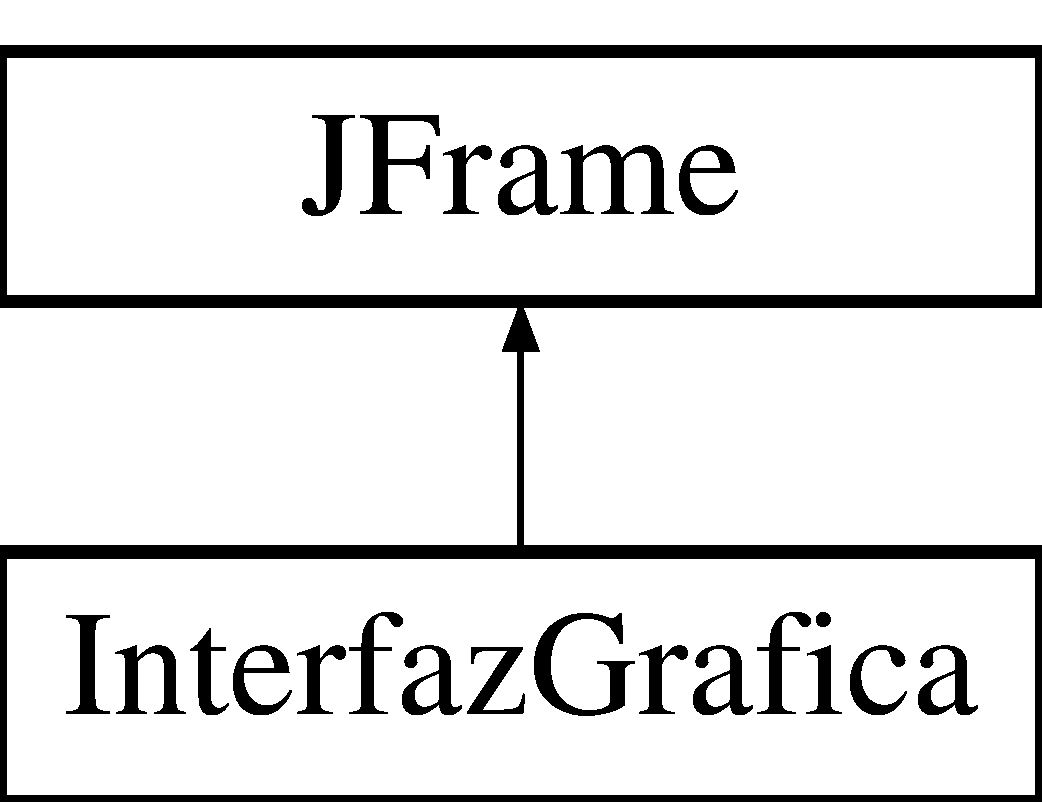
\includegraphics[height=2.000000cm]{class_interfaz_grafica}
\end{center}
\end{figure}
\subsection*{Public Member Functions}
\begin{DoxyCompactItemize}
\item 
\mbox{\hyperlink{class_interfaz_grafica_a3ab695965d5886c0257148cab68974d9}{Interfaz\+Grafica}} (\mbox{\hyperlink{class_tablero}{Tablero}} t, Boolean c)
\begin{DoxyCompactList}\small\item\em Construye una instancia de la Interfaz. \end{DoxyCompactList}\item 
\mbox{\Hypertarget{class_interfaz_grafica_a7b11c3ed50300568a847fa6889939b37}\label{class_interfaz_grafica_a7b11c3ed50300568a847fa6889939b37}} 
void {\bfseries paint} (Graphics g)
\end{DoxyCompactItemize}
\subsection*{Public Attributes}
\begin{DoxyCompactItemize}
\item 
\mbox{\Hypertarget{class_interfaz_grafica_a365ee1e5e4b4dc9a22a93dd4641151bc}\label{class_interfaz_grafica_a365ee1e5e4b4dc9a22a93dd4641151bc}} 
\mbox{\hyperlink{class_tablero}{Tablero}} {\bfseries tablero}
\end{DoxyCompactItemize}


\subsection{Detailed Description}
Esta clase muestra el tablero y permite jugar en el Cuenta con los modos de juego con computadora y 2 jugadores Esta es un frame y recibe interaccion con el usuario mediante el mouse. Este ultimo es el que tiene la informacion de cuando se termina el juego y realiza las operaciones de poner fichas. 

\subsection{Constructor \& Destructor Documentation}
\mbox{\Hypertarget{class_interfaz_grafica_a3ab695965d5886c0257148cab68974d9}\label{class_interfaz_grafica_a3ab695965d5886c0257148cab68974d9}} 
\index{Interfaz\+Grafica@{Interfaz\+Grafica}!Interfaz\+Grafica@{Interfaz\+Grafica}}
\index{Interfaz\+Grafica@{Interfaz\+Grafica}!Interfaz\+Grafica@{Interfaz\+Grafica}}
\subsubsection{\texorpdfstring{Interfaz\+Grafica()}{InterfazGrafica()}}
{\footnotesize\ttfamily Interfaz\+Grafica.\+Interfaz\+Grafica (\begin{DoxyParamCaption}\item[{\mbox{\hyperlink{class_tablero}{Tablero}}}]{t,  }\item[{Boolean}]{c }\end{DoxyParamCaption})}



Construye una instancia de la Interfaz. 


\begin{DoxyParams}{Parameters}
{\em recibe} & el tablero sobre el cual se va a jugar \\
\hline
{\em y} & un booleano que indica si se juega o no contra la computadora. Ademas pone los botones de salir y volver al menu \\
\hline
\end{DoxyParams}


The documentation for this class was generated from the following file\+:\begin{DoxyCompactItemize}
\item 
Interfaz\+Grafica.\+java\end{DoxyCompactItemize}

\hypertarget{class_menu_principal}{}\section{Menu\+Principal Class Reference}
\label{class_menu_principal}\index{Menu\+Principal@{Menu\+Principal}}


La clase del menu principal es la que contiene el main Esta cuenta con las opciones para jugar dso jugadores o solo contra la computadora. Tambien tiene la opcion de entrar a los puntajes y salir del juego.  


Inheritance diagram for Menu\+Principal\+:\begin{figure}[H]
\begin{center}
\leavevmode
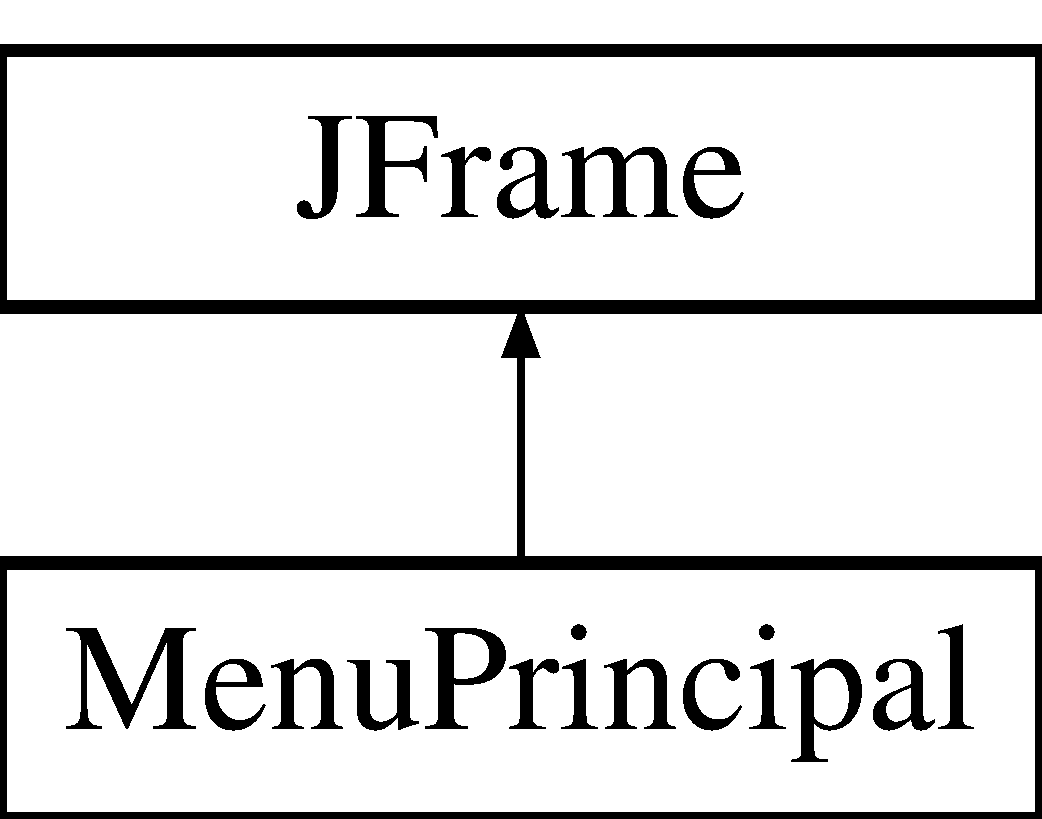
\includegraphics[height=2.000000cm]{class_menu_principal}
\end{center}
\end{figure}
\subsection*{Public Member Functions}
\begin{DoxyCompactItemize}
\item 
\mbox{\Hypertarget{class_menu_principal_abb574127c6a1e0ca6c56f68fc6bb18eb}\label{class_menu_principal_abb574127c6a1e0ca6c56f68fc6bb18eb}} 
\mbox{\hyperlink{class_menu_principal_abb574127c6a1e0ca6c56f68fc6bb18eb}{Menu\+Principal}} ()
\begin{DoxyCompactList}\small\item\em Construye una instancia del menu Esta inicializa los botones. \end{DoxyCompactList}\item 
\mbox{\Hypertarget{class_menu_principal_a68c852495f1ed76cb61f570af9ae7a52}\label{class_menu_principal_a68c852495f1ed76cb61f570af9ae7a52}} 
void {\bfseries paint} (Graphics g)
\end{DoxyCompactItemize}
\subsection*{Static Public Member Functions}
\begin{DoxyCompactItemize}
\item 
\mbox{\Hypertarget{class_menu_principal_a9331983545333d10787f7bbe27dc3b1b}\label{class_menu_principal_a9331983545333d10787f7bbe27dc3b1b}} 
static void {\bfseries main} (String args \mbox{[}$\,$\mbox{]})
\end{DoxyCompactItemize}


\subsection{Detailed Description}
La clase del menu principal es la que contiene el main Esta cuenta con las opciones para jugar dso jugadores o solo contra la computadora. Tambien tiene la opcion de entrar a los puntajes y salir del juego. 

The documentation for this class was generated from the following file\+:\begin{DoxyCompactItemize}
\item 
Menu\+Principal.\+java\end{DoxyCompactItemize}

\hypertarget{class_menu_puntajes}{}\section{Menu\+Puntajes Class Reference}
\label{class_menu_puntajes}\index{Menu\+Puntajes@{Menu\+Puntajes}}


Este es el menu que contiene los puntajes cuenta con los botones muestra en la pantalla los puntajes de los 3 distintos tableros.  


Inheritance diagram for Menu\+Puntajes\+:\begin{figure}[H]
\begin{center}
\leavevmode
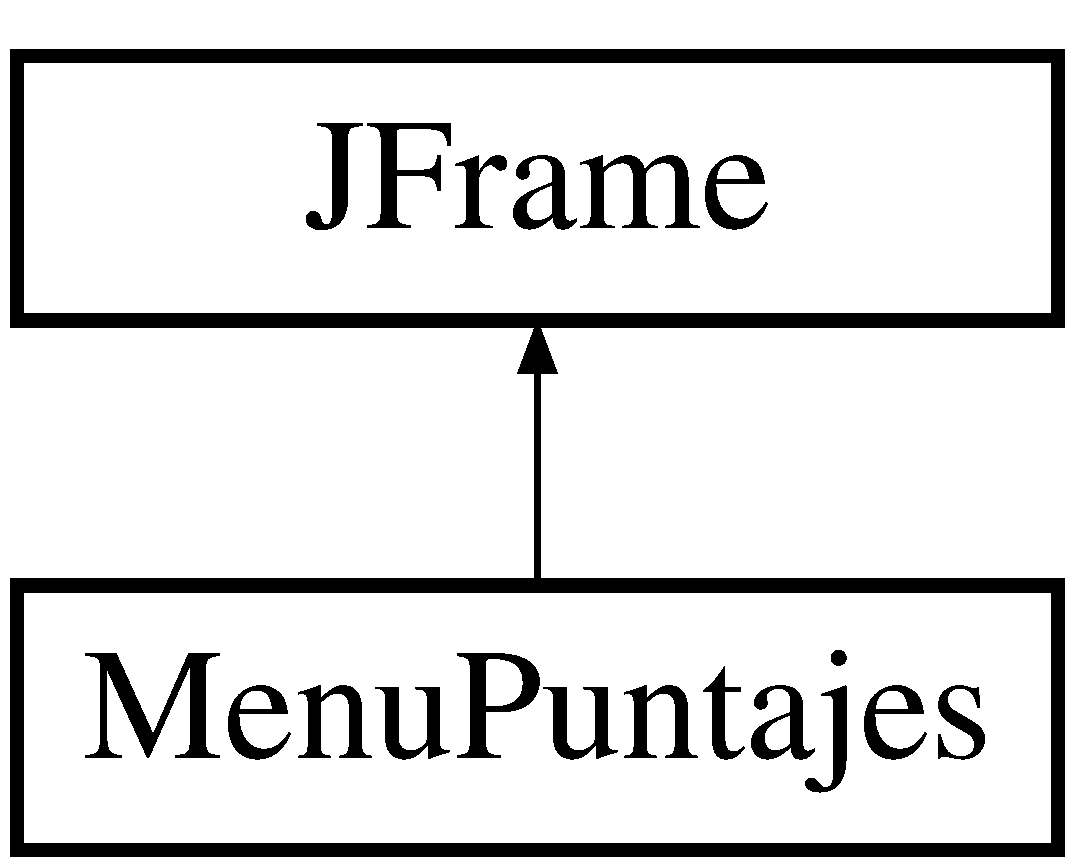
\includegraphics[height=2.000000cm]{class_menu_puntajes}
\end{center}
\end{figure}
\subsection*{Public Member Functions}
\begin{DoxyCompactItemize}
\item 
\mbox{\Hypertarget{class_menu_puntajes_a55f14c668188169b727ab70886036b7c}\label{class_menu_puntajes_a55f14c668188169b727ab70886036b7c}} 
\mbox{\hyperlink{class_menu_puntajes_a55f14c668188169b727ab70886036b7c}{Menu\+Puntajes}} (boolean c)
\begin{DoxyCompactList}\small\item\em Construye una instancia del menu de puntajes esta recibe si es puntajes con o sin computadora y inicializa los botones de atras y salir. \end{DoxyCompactList}\item 
\mbox{\Hypertarget{class_menu_puntajes_a89979e9e1e546e1ae028d860ed19d754}\label{class_menu_puntajes_a89979e9e1e546e1ae028d860ed19d754}} 
void {\bfseries paint} (Graphics g)
\end{DoxyCompactItemize}


\subsection{Detailed Description}
Este es el menu que contiene los puntajes cuenta con los botones muestra en la pantalla los puntajes de los 3 distintos tableros. 

The documentation for this class was generated from the following file\+:\begin{DoxyCompactItemize}
\item 
Menu\+Puntajes.\+java\end{DoxyCompactItemize}

\hypertarget{class_menu_tableros}{}\section{Menu\+Tableros Class Reference}
\label{class_menu_tableros}\index{Menu\+Tableros@{Menu\+Tableros}}


Esta clase muestra las opciones de los 3 tableros para elegir en cual jugar.  


Inheritance diagram for Menu\+Tableros\+:\begin{figure}[H]
\begin{center}
\leavevmode
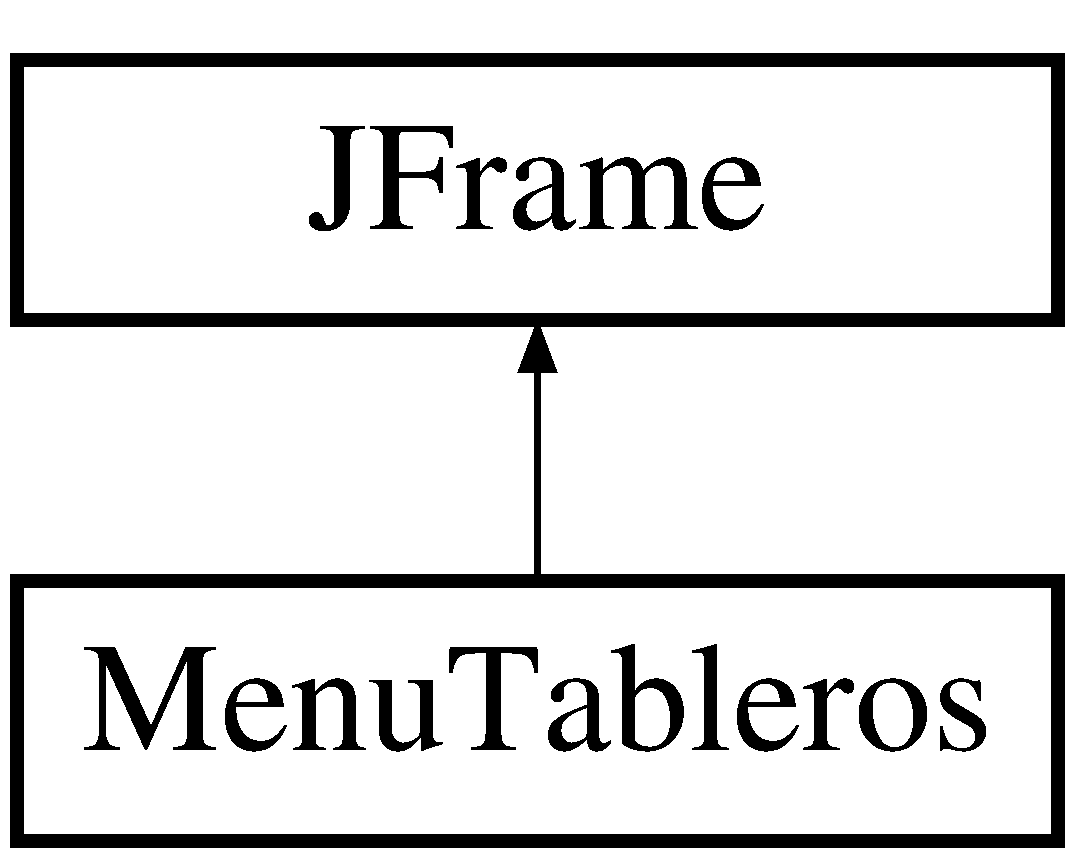
\includegraphics[height=2.000000cm]{class_menu_tableros}
\end{center}
\end{figure}
\subsection*{Public Member Functions}
\begin{DoxyCompactItemize}
\item 
\mbox{\hyperlink{class_menu_tableros_a1cb8d60a9dd5696979e8388106845bcd}{Menu\+Tableros}} (boolean c)
\begin{DoxyCompactList}\small\item\em Construye una instancia de la Interfaz. \end{DoxyCompactList}\item 
\mbox{\Hypertarget{class_menu_tableros_abca0554cdf42215b9bc20c16c0a52f2d}\label{class_menu_tableros_abca0554cdf42215b9bc20c16c0a52f2d}} 
void {\bfseries paint} (Graphics g)
\end{DoxyCompactItemize}


\subsection{Detailed Description}
Esta clase muestra las opciones de los 3 tableros para elegir en cual jugar. 

\subsection{Constructor \& Destructor Documentation}
\mbox{\Hypertarget{class_menu_tableros_a1cb8d60a9dd5696979e8388106845bcd}\label{class_menu_tableros_a1cb8d60a9dd5696979e8388106845bcd}} 
\index{Menu\+Tableros@{Menu\+Tableros}!Menu\+Tableros@{Menu\+Tableros}}
\index{Menu\+Tableros@{Menu\+Tableros}!Menu\+Tableros@{Menu\+Tableros}}
\subsubsection{\texorpdfstring{Menu\+Tableros()}{MenuTableros()}}
{\footnotesize\ttfamily Menu\+Tableros.\+Menu\+Tableros (\begin{DoxyParamCaption}\item[{boolean}]{c }\end{DoxyParamCaption})}



Construye una instancia de la Interfaz. 


\begin{DoxyParams}{Parameters}
{\em Recibe} & booleano que indica si se juega o no contra la computadora. Ademas pone los botones delos tableros, salir y volver al menu. \\
\hline
\end{DoxyParams}


The documentation for this class was generated from the following file\+:\begin{DoxyCompactItemize}
\item 
Menu\+Tableros.\+java\end{DoxyCompactItemize}

\hypertarget{class_puntaje}{}\section{Puntaje Class Reference}
\label{class_puntaje}\index{Puntaje@{Puntaje}}


Información de una fila en cada tabla de puntajes.  


Inheritance diagram for Puntaje\+:\begin{figure}[H]
\begin{center}
\leavevmode
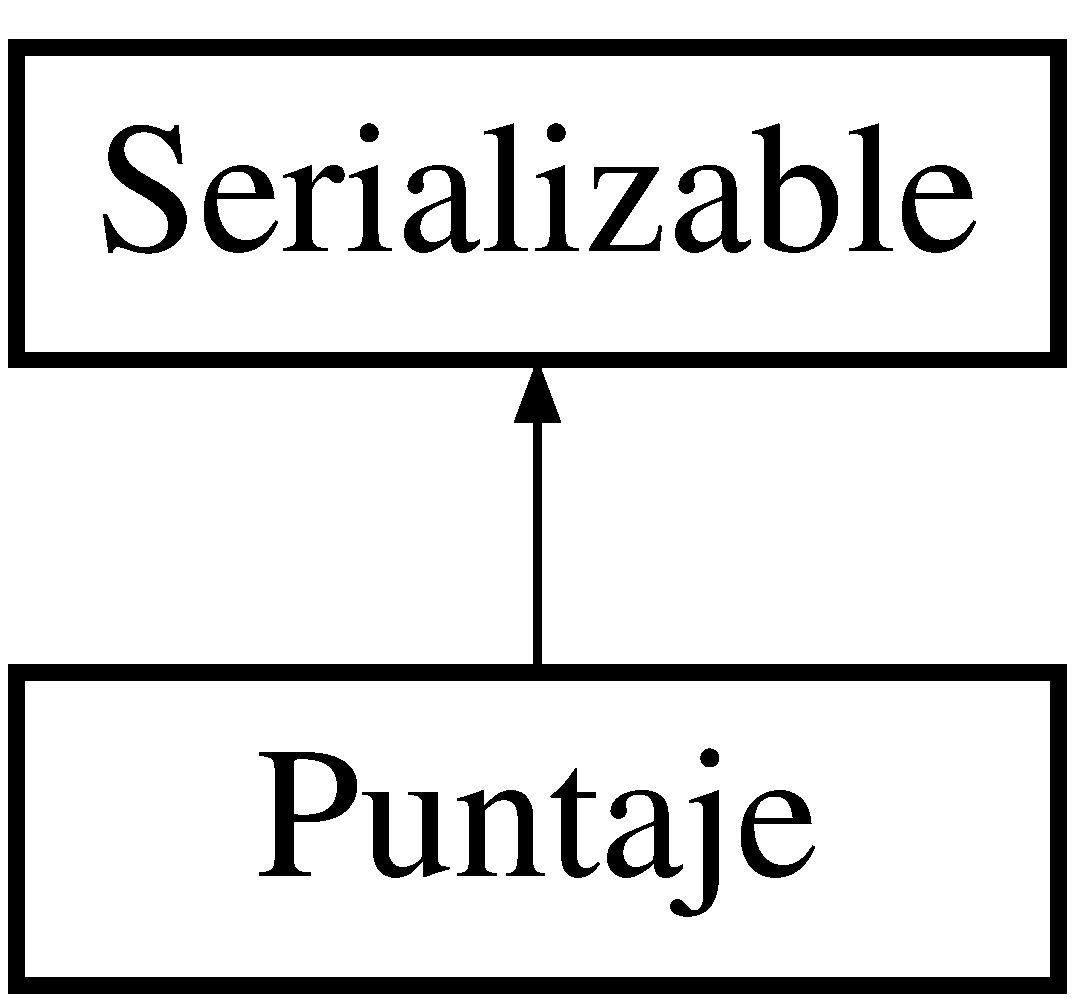
\includegraphics[height=2.000000cm]{class_puntaje}
\end{center}
\end{figure}
\subsection*{Public Member Functions}
\begin{DoxyCompactItemize}
\item 
\mbox{\hyperlink{class_puntaje_a66330c08cb2e451370489d26b0ef20c1}{Puntaje}} (String nombre, int puntos, int tamano)
\begin{DoxyCompactList}\small\item\em Construye una fila de datos con la información indicada. \end{DoxyCompactList}\item 
\mbox{\Hypertarget{class_puntaje_a5264405a77ab9884e8f3a4a9117d4273}\label{class_puntaje_a5264405a77ab9884e8f3a4a9117d4273}} 
String {\bfseries get\+Nombre} ()
\item 
\mbox{\Hypertarget{class_puntaje_a74f9d10f035df4ae417094b6b0d06839}\label{class_puntaje_a74f9d10f035df4ae417094b6b0d06839}} 
int {\bfseries get\+Puntos} ()
\item 
\mbox{\Hypertarget{class_puntaje_a9657b9127f63f2ad40ea36c2b7dfc374}\label{class_puntaje_a9657b9127f63f2ad40ea36c2b7dfc374}} 
int {\bfseries get\+Tamano} ()
\item 
\mbox{\Hypertarget{class_puntaje_a847332131e62ee45ace5d1e6b89ef275}\label{class_puntaje_a847332131e62ee45ace5d1e6b89ef275}} 
String {\bfseries to\+String} ()
\end{DoxyCompactItemize}


\subsection{Detailed Description}
Información de una fila en cada tabla de puntajes. 

Esta clase es un contenedor de la información de cada fila en las tablas puntajes. 

\subsection{Constructor \& Destructor Documentation}
\mbox{\Hypertarget{class_puntaje_a66330c08cb2e451370489d26b0ef20c1}\label{class_puntaje_a66330c08cb2e451370489d26b0ef20c1}} 
\index{Puntaje@{Puntaje}!Puntaje@{Puntaje}}
\index{Puntaje@{Puntaje}!Puntaje@{Puntaje}}
\subsubsection{\texorpdfstring{Puntaje()}{Puntaje()}}
{\footnotesize\ttfamily Puntaje.\+Puntaje (\begin{DoxyParamCaption}\item[{String}]{nombre,  }\item[{int}]{puntos,  }\item[{int}]{tamano }\end{DoxyParamCaption})}



Construye una fila de datos con la información indicada. 


\begin{DoxyParams}{Parameters}
{\em nombre} & El nombre del jugador. El nombre es truncado a 15 caracteres. \\
\hline
{\em puntos} & Los puntos que obtuvo. \\
\hline
{\em tamano} & El modo de juego donde hizo los puntos (el tamaño del tablero). \\
\hline
\end{DoxyParams}


The documentation for this class was generated from the following file\+:\begin{DoxyCompactItemize}
\item 
Puntaje.\+java\end{DoxyCompactItemize}

\hypertarget{class_puntajes_computadora_o_jugador}{}\section{Puntajes\+Computadora\+O\+Jugador Class Reference}
\label{class_puntajes_computadora_o_jugador}\index{Puntajes\+Computadora\+O\+Jugador@{Puntajes\+Computadora\+O\+Jugador}}
Inheritance diagram for Puntajes\+Computadora\+O\+Jugador\+:\begin{figure}[H]
\begin{center}
\leavevmode
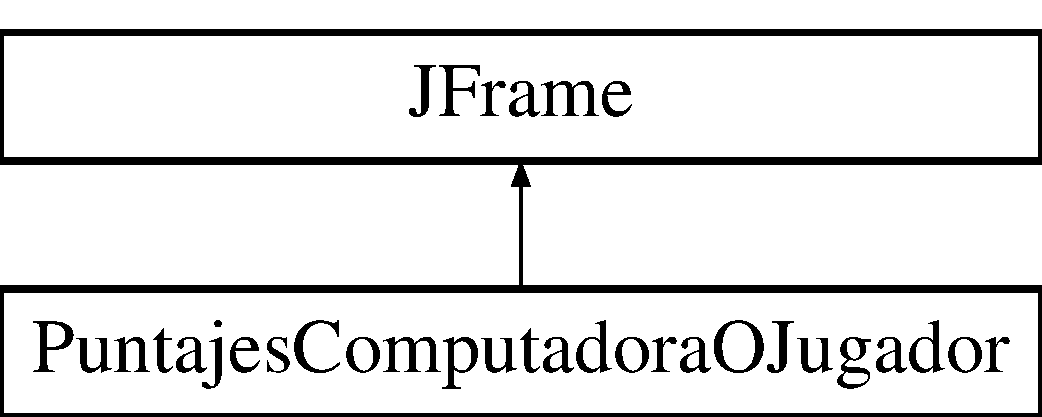
\includegraphics[height=2.000000cm]{class_puntajes_computadora_o_jugador}
\end{center}
\end{figure}
\subsection*{Public Member Functions}
\begin{DoxyCompactItemize}
\item 
\mbox{\Hypertarget{class_puntajes_computadora_o_jugador_a34374109c4e103fb5c920f87a3cd9b95}\label{class_puntajes_computadora_o_jugador_a34374109c4e103fb5c920f87a3cd9b95}} 
\mbox{\hyperlink{class_puntajes_computadora_o_jugador_a34374109c4e103fb5c920f87a3cd9b95}{Puntajes\+Computadora\+O\+Jugador}} ()
\begin{DoxyCompactList}\small\item\em Construye una instancia del menu. A�ade los botones para elegir si ver puntajes de computadora o 2 jugadores. \end{DoxyCompactList}\item 
\mbox{\Hypertarget{class_puntajes_computadora_o_jugador_a42855886c37db7173ce6db27967159cb}\label{class_puntajes_computadora_o_jugador_a42855886c37db7173ce6db27967159cb}} 
void {\bfseries paint} (Graphics g)
\end{DoxyCompactItemize}


The documentation for this class was generated from the following file\+:\begin{DoxyCompactItemize}
\item 
Puntajes\+Computadora\+O\+Jugador.\+java\end{DoxyCompactItemize}

\hypertarget{class_tablero}{}\section{Tablero Class Reference}
\label{class_tablero}\index{Tablero@{Tablero}}


El tablero donde se almacena la información del juego.  


\subsection*{Public Member Functions}
\begin{DoxyCompactItemize}
\item 
\mbox{\hyperlink{class_tablero_ac92adc2bd5f2ed16d8ee121523956c49}{Tablero}} (int tamano)
\begin{DoxyCompactList}\small\item\em Inicializa el tablero con el tamaño indicado y las cuatro fichas centrales. \end{DoxyCompactList}\item 
\mbox{\Hypertarget{class_tablero_af506d72b2430b8e1068ac16e50a324a6}\label{class_tablero_af506d72b2430b8e1068ac16e50a324a6}} 
int \mbox{\hyperlink{class_tablero_af506d72b2430b8e1068ac16e50a324a6}{get\+Tamano}} ()
\begin{DoxyCompactList}\small\item\em Retorna el tamaño del tablero. \end{DoxyCompactList}\item 
int \mbox{\hyperlink{class_tablero_af35697b272eb9fa8478867da8ce49caf}{cantidad\+Negras}} ()
\begin{DoxyCompactList}\small\item\em Cuenta la cantidad de fichas negras. \end{DoxyCompactList}\item 
int \mbox{\hyperlink{class_tablero_a8467113a62a739be46f6a17ce876e97e}{cantidad\+Blancas}} ()
\begin{DoxyCompactList}\small\item\em Cuenta la cantidad de fichas blancas. \end{DoxyCompactList}\item 
int \mbox{\hyperlink{class_tablero_a885e7de2aeb202acd70c1ac8896ad1c1}{get\+Color}} (int fila, int columna)
\begin{DoxyCompactList}\small\item\em Devuelve el color de un cuadro en el tablero. \end{DoxyCompactList}\item 
boolean \mbox{\hyperlink{class_tablero_afbf952c36374051ba9d9a007ad2c673d}{puede\+Poner}} (int color, int fila, int columna)
\begin{DoxyCompactList}\small\item\em Indica si se puede colocar una ficha de un color dado en un cuadro del tablero. \end{DoxyCompactList}\item 
boolean \mbox{\hyperlink{class_tablero_a0b225d49792c0db4742c1e6aea909647}{existen\+Jugadas}} (int color)
\begin{DoxyCompactList}\small\item\em Indica si existen jugadas válidas para un color dado en algún lugar del tablero. \end{DoxyCompactList}\item 
void \mbox{\hyperlink{class_tablero_a22addb609780226aa6371c818b4d5a12}{poner}} (int color, int fila, int columna)
\begin{DoxyCompactList}\small\item\em Coloca la pieza del color indicado en la posición indicada. \end{DoxyCompactList}\end{DoxyCompactItemize}
\subsection*{Static Public Member Functions}
\begin{DoxyCompactItemize}
\item 
static int \mbox{\hyperlink{class_tablero_a0cdaee39a2bd8bd7fa59b2c19958650c}{color\+Opuesto}} (int color)
\begin{DoxyCompactList}\small\item\em Invierte el color de N\+E\+G\+RO a B\+L\+A\+N\+CO y viceversa. \end{DoxyCompactList}\end{DoxyCompactItemize}
\subsection*{Static Public Attributes}
\begin{DoxyCompactItemize}
\item 
\mbox{\Hypertarget{class_tablero_a0ef9ac784851be4a99984b6a2dcede58}\label{class_tablero_a0ef9ac784851be4a99984b6a2dcede58}} 
static final int \mbox{\hyperlink{class_tablero_a0ef9ac784851be4a99984b6a2dcede58}{N\+E\+G\+RO}} =1
\begin{DoxyCompactList}\small\item\em Representa una casilla con una ficha negra. \end{DoxyCompactList}\item 
\mbox{\Hypertarget{class_tablero_a28a1e0a4c4362e5cbcb2505b660c6855}\label{class_tablero_a28a1e0a4c4362e5cbcb2505b660c6855}} 
static final int \mbox{\hyperlink{class_tablero_a28a1e0a4c4362e5cbcb2505b660c6855}{B\+L\+A\+N\+CO}} =-\/1
\begin{DoxyCompactList}\small\item\em Representa una casilla con una ficha blanca. \end{DoxyCompactList}\item 
\mbox{\Hypertarget{class_tablero_abbd0033f1dfd3e3d30c1b11472d057c9}\label{class_tablero_abbd0033f1dfd3e3d30c1b11472d057c9}} 
static final int \mbox{\hyperlink{class_tablero_abbd0033f1dfd3e3d30c1b11472d057c9}{V\+A\+C\+IO}} =0
\begin{DoxyCompactList}\small\item\em Representa una casilla vacía. \end{DoxyCompactList}\end{DoxyCompactItemize}


\subsection{Detailed Description}
El tablero donde se almacena la información del juego. 

Cada instancia de esta clase se inicializa especificando el tamaño (cantidad de filas y columnas). Automáticamente se colocan las cuatro fichas centrales.

El tablero consiste en una matriz cuadrada con los tres posibles valores N\+E\+G\+RO, B\+L\+A\+N\+CO y V\+A\+C\+IO.

Esta clase se encarga de indicar si se puede o no colocar una ficha en un lugar especificado y poner las fichas cuando se le indica (realizando las sustituciones de las piezas que come). 

\subsection{Constructor \& Destructor Documentation}
\mbox{\Hypertarget{class_tablero_ac92adc2bd5f2ed16d8ee121523956c49}\label{class_tablero_ac92adc2bd5f2ed16d8ee121523956c49}} 
\index{Tablero@{Tablero}!Tablero@{Tablero}}
\index{Tablero@{Tablero}!Tablero@{Tablero}}
\subsubsection{\texorpdfstring{Tablero()}{Tablero()}}
{\footnotesize\ttfamily Tablero.\+Tablero (\begin{DoxyParamCaption}\item[{int}]{tamano }\end{DoxyParamCaption})}



Inicializa el tablero con el tamaño indicado y las cuatro fichas centrales. 


\begin{DoxyParams}{Parameters}
{\em tamano} & El tamaño del tablero. \\
\hline
\end{DoxyParams}


\subsection{Member Function Documentation}
\mbox{\Hypertarget{class_tablero_a8467113a62a739be46f6a17ce876e97e}\label{class_tablero_a8467113a62a739be46f6a17ce876e97e}} 
\index{Tablero@{Tablero}!cantidad\+Blancas@{cantidad\+Blancas}}
\index{cantidad\+Blancas@{cantidad\+Blancas}!Tablero@{Tablero}}
\subsubsection{\texorpdfstring{cantidad\+Blancas()}{cantidadBlancas()}}
{\footnotesize\ttfamily int Tablero.\+cantidad\+Blancas (\begin{DoxyParamCaption}{ }\end{DoxyParamCaption})}



Cuenta la cantidad de fichas blancas. 

Itera sobre los cuadros del tablero y retorna la cantidad de fichas blancas.

\begin{DoxyReturn}{Returns}
La cantidad de fichas blancas sobre el tablero. 
\end{DoxyReturn}
\mbox{\Hypertarget{class_tablero_af35697b272eb9fa8478867da8ce49caf}\label{class_tablero_af35697b272eb9fa8478867da8ce49caf}} 
\index{Tablero@{Tablero}!cantidad\+Negras@{cantidad\+Negras}}
\index{cantidad\+Negras@{cantidad\+Negras}!Tablero@{Tablero}}
\subsubsection{\texorpdfstring{cantidad\+Negras()}{cantidadNegras()}}
{\footnotesize\ttfamily int Tablero.\+cantidad\+Negras (\begin{DoxyParamCaption}{ }\end{DoxyParamCaption})}



Cuenta la cantidad de fichas negras. 

Itera sobre los cuadros del tablero y retorna la cantidad de fichas negras.

\begin{DoxyReturn}{Returns}
La cantidad de fichas negras sobre el tablero. 
\end{DoxyReturn}
\mbox{\Hypertarget{class_tablero_a0cdaee39a2bd8bd7fa59b2c19958650c}\label{class_tablero_a0cdaee39a2bd8bd7fa59b2c19958650c}} 
\index{Tablero@{Tablero}!color\+Opuesto@{color\+Opuesto}}
\index{color\+Opuesto@{color\+Opuesto}!Tablero@{Tablero}}
\subsubsection{\texorpdfstring{color\+Opuesto()}{colorOpuesto()}}
{\footnotesize\ttfamily static int Tablero.\+color\+Opuesto (\begin{DoxyParamCaption}\item[{int}]{color }\end{DoxyParamCaption})\hspace{0.3cm}{\ttfamily [static]}}



Invierte el color de N\+E\+G\+RO a B\+L\+A\+N\+CO y viceversa. 


\begin{DoxyParams}{Parameters}
{\em color} & El color que se desea invertir. \\
\hline
\end{DoxyParams}
\begin{DoxyReturn}{Returns}
Si color es B\+L\+A\+N\+CO retorna N\+E\+G\+RO. Si color es N\+E\+G\+RO retorna B\+L\+A\+N\+CO. En cualquier otro caso retorna V\+A\+C\+IO. 
\end{DoxyReturn}
\mbox{\Hypertarget{class_tablero_a0b225d49792c0db4742c1e6aea909647}\label{class_tablero_a0b225d49792c0db4742c1e6aea909647}} 
\index{Tablero@{Tablero}!existen\+Jugadas@{existen\+Jugadas}}
\index{existen\+Jugadas@{existen\+Jugadas}!Tablero@{Tablero}}
\subsubsection{\texorpdfstring{existen\+Jugadas()}{existenJugadas()}}
{\footnotesize\ttfamily boolean Tablero.\+existen\+Jugadas (\begin{DoxyParamCaption}\item[{int}]{color }\end{DoxyParamCaption})}



Indica si existen jugadas válidas para un color dado en algún lugar del tablero. 

Esta función itera sobre cada casilla del tablero, invocando al método \mbox{\hyperlink{class_tablero_afbf952c36374051ba9d9a007ad2c673d}{puede\+Poner()}} y retorna true si se puede poner en algún lugar y false si no.


\begin{DoxyParams}{Parameters}
{\em color} & El color de la ficha que se quiere colocar. \\
\hline
\end{DoxyParams}
\begin{DoxyReturn}{Returns}
true si existe alguna jugada en el tablero, false si no. 
\end{DoxyReturn}
\mbox{\Hypertarget{class_tablero_a885e7de2aeb202acd70c1ac8896ad1c1}\label{class_tablero_a885e7de2aeb202acd70c1ac8896ad1c1}} 
\index{Tablero@{Tablero}!get\+Color@{get\+Color}}
\index{get\+Color@{get\+Color}!Tablero@{Tablero}}
\subsubsection{\texorpdfstring{get\+Color()}{getColor()}}
{\footnotesize\ttfamily int Tablero.\+get\+Color (\begin{DoxyParamCaption}\item[{int}]{fila,  }\item[{int}]{columna }\end{DoxyParamCaption})}



Devuelve el color de un cuadro en el tablero. 


\begin{DoxyParams}{Parameters}
{\em fila} & La fila de donde se quiere obtener el color. \\
\hline
{\em columna} & La columna de donde se quiere obtener el color. \\
\hline
\end{DoxyParams}
\begin{DoxyReturn}{Returns}
Retorna alguno de los valores \mbox{\hyperlink{class_tablero_abbd0033f1dfd3e3d30c1b11472d057c9}{Tablero.\+V\+A\+C\+IO}}, \mbox{\hyperlink{class_tablero_a0ef9ac784851be4a99984b6a2dcede58}{Tablero.\+N\+E\+G\+RO}} o \mbox{\hyperlink{class_tablero_a28a1e0a4c4362e5cbcb2505b660c6855}{Tablero.\+B\+L\+A\+N\+CO}}, según corresponda. 
\end{DoxyReturn}
\mbox{\Hypertarget{class_tablero_a22addb609780226aa6371c818b4d5a12}\label{class_tablero_a22addb609780226aa6371c818b4d5a12}} 
\index{Tablero@{Tablero}!poner@{poner}}
\index{poner@{poner}!Tablero@{Tablero}}
\subsubsection{\texorpdfstring{poner()}{poner()}}
{\footnotesize\ttfamily void Tablero.\+poner (\begin{DoxyParamCaption}\item[{int}]{color,  }\item[{int}]{fila,  }\item[{int}]{columna }\end{DoxyParamCaption})}



Coloca la pieza del color indicado en la posición indicada. 

Coloca la pieza del color indicado en la posición indicada y sustituye las piezas que se come por el nuevo color. Invocar este método en un lugar inválido (fuera del tablero o que no admita una jugada válida) resulta en una excepción.


\begin{DoxyParams}{Parameters}
{\em color} & El color de la ficha que se desea poner. \\
\hline
{\em fila} & La fila de la casilla. \\
\hline
{\em columna} & La columna de la casilla. \\
\hline
\end{DoxyParams}
\mbox{\Hypertarget{class_tablero_afbf952c36374051ba9d9a007ad2c673d}\label{class_tablero_afbf952c36374051ba9d9a007ad2c673d}} 
\index{Tablero@{Tablero}!puede\+Poner@{puede\+Poner}}
\index{puede\+Poner@{puede\+Poner}!Tablero@{Tablero}}
\subsubsection{\texorpdfstring{puede\+Poner()}{puedePoner()}}
{\footnotesize\ttfamily boolean Tablero.\+puede\+Poner (\begin{DoxyParamCaption}\item[{int}]{color,  }\item[{int}]{fila,  }\item[{int}]{columna }\end{DoxyParamCaption})}



Indica si se puede colocar una ficha de un color dado en un cuadro del tablero. 

Este método verifica que la casilla donde se quiere colocar la ficha esté vacía y que la jugada sea válida, es decir, que pueda comer piezas del color opuesto al colocar la ficha.


\begin{DoxyParams}{Parameters}
{\em color} & El color de la ficha que se quiere poner. \\
\hline
{\em fila} & La fila de donde se quiere obtener el color. \\
\hline
{\em columna} & La columna de donde se quiere obtener el color. \\
\hline
\end{DoxyParams}
\begin{DoxyReturn}{Returns}
true si puede se puede poner una ficha del \textquotesingle{}color\textquotesingle{} en el lugar especificado 
\end{DoxyReturn}


The documentation for this class was generated from the following file\+:\begin{DoxyCompactItemize}
\item 
Tablero.\+java\end{DoxyCompactItemize}

%--- End generated contents ---

% Index
\backmatter
\newpage
\phantomsection
\clearemptydoublepage
\addcontentsline{toc}{chapter}{Index}
\printindex

\end{document}
